\documentclass[preprint]{elsarticle}
\usepackage[latin1]{inputenc}
\usepackage[english]{babel}
%\usepackage[T1]{fontenc}
%\usepackage{textcomp}
\usepackage{graphicx}
\usepackage{color}
%\usepackage{setspace}
\usepackage{url}

\begin{document}

\begin{frontmatter}

%%%%%%%%%%%%%%%%%%%%%%%%%%%%%%%   TITLE   %%%%%%%%%%%%%%%%%%%%%%%%%%%%%%%

\title{Nowcasting traffic}


%%%%%%%%%%%%%%%%%%%%%%%%%%%%%%%   AUTHORS   %%%%%%%%%%%%%%%%%%%%%%%%%%%%%%%

\author{A.J. Fern�ndez-Ares$^1$, A.M. Mora$^1$, M.G. Arenas$^1$, P. Garc�a-Sanchez$^1$, G. Romero$^1$, V. Rivas$^2$, P.A. Castillo$^1$, J.J. Merelo$^1$}
\ead{\{antares, amorag, mgarenas, pablogarcia, gustavo, pacv, jmerelo\}@ugr.es, vrivas@ujaes.es}
\address{$^1$ Departamento de Arquitectura y Tecnolog�a de Computadores.\\ ETSIIT - CITIC. University of Granada, Spain\\
$^2$ Departamento de Inform�tica. EPS. Universidad de Ja�n, Spain}


\begin{abstract}
Traffic flow measurement methods suffer must keep a balance between being comprehensive, expensive and cumbersome, such as traffic spirals, or being cheap, mobile but missing some counts.
In the framework of a smart city project, our group has been
developing MOBYWIT, a device that detects unique Bluetooth and Wifi
MACs and thus is able to measure their traffic, but also to identify
uniquely bearers so that we can find out the actual path a particular
vehicle has followed. However, not all vehicles have bluetooth devices
and the relation between them and the actual number of vehicles varies
along the day, the time of the day and characteristics of the road. 
In this work our objective is to "nowcast", that is, to predict, using
all available information, the real number of vehicles given that we
have the number of vehicles bearing a wireless device. We will use
classic and neural network techniques on data gathered in
installations where we have both kind of devices, MOBYWIT and spirals,
to try and find out some rules and give a more accurate estimate of
the real number of cars in a particular road. 
\end{abstract}

%
%%%%%%%%%%%%%%%%%%%%%%%%%%%%%%%%%   KEYWORDS   %%%%%%%%%%%%%%%%%%%%%%%%%%%%%%%%%
%
\begin{keyword}
Smart traffic \sep Transit indicators \sep Traffic forecast \sep Mobility analysis \sep Smart City \sep Internet of Things
\end{keyword}

\end{frontmatter}


%-------------------------------------------------------------------------------
%%%%%%%%%%%%%%%%%%%%%%%%%%%%%%%   INTRODUCTION   %%%%%%%%%%%%%%%%%%%%%%%%%%%%%%%
%-------------------------------------------------------------------------------

\section{Introduction}
\label{sec:intro}

Monitoring traffic and knowing the exact amount of vehicles that are
occupying a street in a particular moment is an issue where you have
to balance accuracy and price or convenience. Spirals embedded on the
road can give you the exact number of vehicles and even its type;
however, besides being expensive per se, the road has to be opened
and re-asphalted to install them so they cannot be intalled at short
notice. On the other hand, devices such as Mobywit
\cite{DBLP:conf/smartct/Fernandez-AresA16}, which use some feature of
vehicles such as the emitting devices in them, only count part of the
devices and thus their accuracy is limited; incidentally, systems such
as the one used by Google Maps also rely on mobile devices
transmitting their location and thus do not cover the totality of
vehicles.

On the other hand, the accurate knowledge of the amount of traffic is
direly needed in the context of Smart Cities in order to avoid
congestions and also be able to plan routes in advance. In this
context, a solution can be using the less-acurate devices, which can
be deployed in a massive amount of places, to {\em now-cast}, that it,
predict, the actual traffic passing by a particular point in that
precise moment. 

In this paper we will use data collected in the course of the PETRA
project to find out, from available data, the actual vehicle count in
a place. We will use standard and bioinspired methods, and try to find
what could be the best option for the volume and type of data
available. Data, as well as its processing, is available in a GitHub
repository as part of the Open Science policy of our group. 

The rest of the work is structured as follows. Section \ref{sec:soa}
presents the background and state of the art. Then, our monitoring device is introduced in Section
\ref{sec:mobywit}. The results on trying to use different prediction
methods are described in section 
Finally, Section \ref{sec:conclusions} plots the conclusions that we
have reached in the work. 


%----------------------------------------------------------------------------
%%%%%%%%%%%%%%%%%%%%%%%%%%%%%   STATE OF THE ART  %%%%%%%%%%%%%%%%%%%%%%%%%%%
%----------------------------------------------------------------------------


\section{Background and state of the art}
\label{sec:soa}

Nowcasting is just a way of predicting the value of data, and thus is not really a new methodology. However, as far as we have been able to find out, it has not been applied to vehicle traffic in the way we do in this paper. In \cite{hanabusa2013development} a model is used to nowcast traffic, instead of partial measurements, and in \cite{scharsching1996nowcasting} road conditions are predicted; in fact, many of the nowcasting applications are related to weather and merge data from different sources in order to predict with a certan spatial accuracy weather conditions.

Our previous work has been mainly devoted to the design and description of the monitoring device itself \cite{DBLP:conf/smartct/Fernandez-AresA16}. In this paper, after describing the system in the next section, we will use available data to predict real traffic. 


%------------------------------------------------------------------------------
%%%%%%%%%%%%%%%%%%%%%%%%%%%%%%%%%%  MOBYWIT  %%%%%%%%%%%%%%%%%%%%%%%%%%%%%%%%%%
%------------------------------------------------------------------------------

\section{MOBYWIT}
\label{sec:mobywit}

The proposed device, which we call MOBYWIT (Mobility monitoring by Wireless Tracking)  is a single-board computer, based on the Raspberry
Pi\footnote{https://es.wikipedia.org/wiki/Raspberry\_Pi}. It includes
BT and WiFi devices connected via USB and configured in monitor mode
so that they can scan the radioelectric space searching for BT devices
and beacon frames (for WiFi).

In every device the monitoring system is formed by a closely coupled
hardware and software layer. The device has to be connected to the
Internet and stores data in the cloud. The software architecture of the system is shown in Figure \ref{fig:mobywit}. 

\begin{figure}[ht]
	\begin{center}
		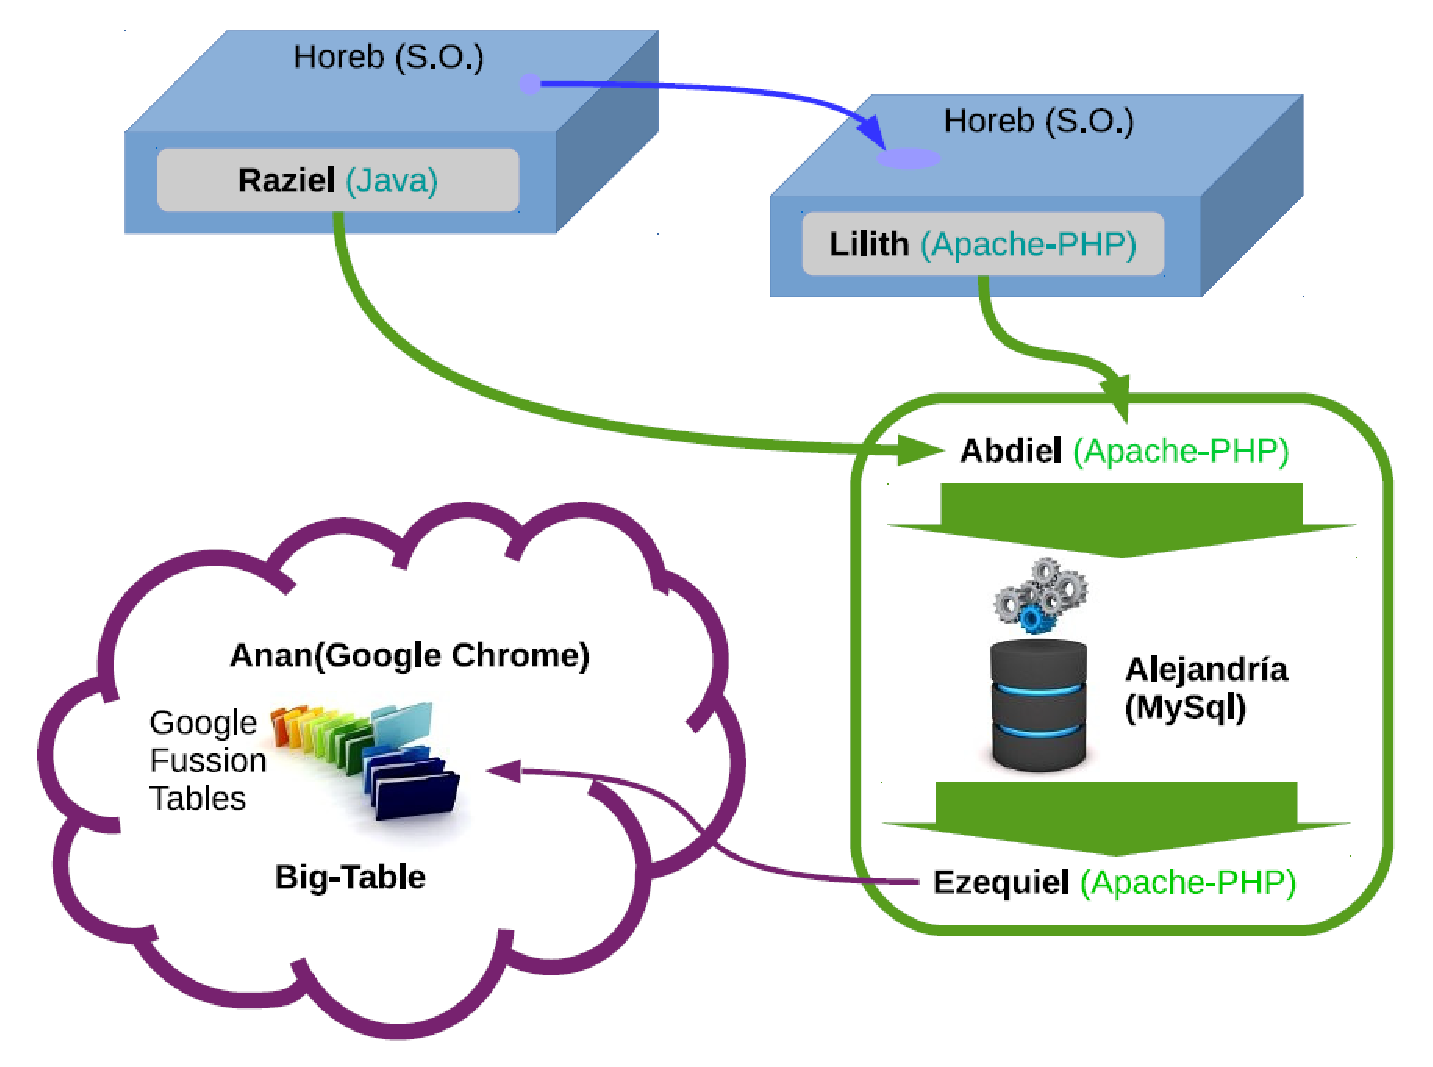
\includegraphics[scale=0.4]{imgs/mobywit.eps}
		\caption{MOBYWIT Monitoring system architecture}
	\label{fig:mobywit}
	\end{center}
\end{figure}

Figure \ref{fig:mobywit} shows the six main parts in the software
layer of the system, which are unidirectionally connected by a strict
data flow. These parts perform the following functions:
\begin{itemize}

\item \textit{Raziel} is in charge of the detection of BT and WiFi
  devices as well as of their identification, that is, extracting and
  encrypting the MAC,  as well as the periodic submission of this information
  to the server. It runs on the device and has been implemented in
  Java.

\item \textit{Lilith} acts as a gateway between the network of devices
  and the server, enabling the communications between nodes and between them and external networks. This component is also run on every device and implemented in PHP.

\item \textit{Abdiel}: This component implements a set of services for accessing the devices from `outside' (mainly for activate/deactivate or update them). In addition, it performs the storage of gathered data (in blocks) in the server database. It is also implemented in PHP.

\item \textit{Alejandr�a} is the database managing subsystem, a MySQL
  instance placed in a local server. It is optimised using b-tree
  indexes, stored procedures, table partitioning and temporally memory
  tables to provide a close to real-time processing and data service. 

\item \textit{Ezequiel} is responsible for the publication of data in
  a cloud-based storage. It includes data mining, machine learning and
  forecasting techniques that act on the data in order to publish
  interesting or useful information about them. 

\item \textit{Anan} is the cloud-based storage and services. It is
  based on Google technology, storing the data in a NoSQL format by
  means of Google Fusion Tables. It also offers advanced visualisation
  methods to be more usable and attractive to the end-user of the
  system. 

\end{itemize}

In addition the device runs a customized Operating System, called
\textit{Horeb}, a modification of the original Raspbian 3.10.24,
adapted by us to be more robust (to power failures, for instance) and
reliable.

There are several configuration parameters in the system, which set
important parts of the functionality, such as the intensity threshold
to collect a received WiFi signal, or time limits to consider a device
as obsolete or out of the range of the device. 

Every detected `pass-by' or mobility `event' is associated with a
detection time, obtained by NTP (Network Time Protocol). These
`events' are stored initially in the device's memory, but after some
time (also set in a parameter) the information is sent, in blocks, to
the server, to avoid an overuse/saturation of the network and also
save bandwidth.

Fron the point of view of this paper, MOBYWIT will collect the number
of devices detected in a particular period of time; so the data we
will have will be a timestamp and a vehicle count. 

\section{Nowcasting traffic}
\label{sec:nowcasting}

Our intention in this paper, and particularly in this section, is to
show that, in fact, there is a high correlation between the number of
vehicles detected and the actual number of vehicles. In order to check
it, the national traffic directorate made available data from their
own spirals, situated near or in the same place as our MOBYWIT. This
data is available from the same repository as this paper,
\url{https://github.com/geneura-papers/nowcasting-traffic}. These data
are from a single month in a single year, and only during 3 hours,
although we have different days the week. The data is not too
comprehensive, but at least gives us an idea of how the existing
factors might influence the outcome. 


One of the things we will have to take into account is that our device
only detects WiFi and Bluetooth devices. In the case of vehicles, it
is mainly hands-free BlueeTooth devices. These devices have to be
installed and connected to be detected, unlike WiFi defices that do
not actually need to be activated; however, very few vehicles nowadays
actually include these devices. Only a fraction of vehicles will be
equipped with any of them, and this amount will change with the time
of the day and also the type of road; while you might expect many more
hands-free devices in urban areas, there might not be as many in rural
areas. Probably the time of the day and the type of traffic,
commuters, services or professional traffic will also present a very
different profile. While commuters might have a lower amount of BT
devices, services or professional will almost always have one. That is
why even as we know that it will always be a fraction, the actual
number will change depending on many different factors. 

In the next subsection we will use only the number of detected
vehicles for nowcasting. In Subsection \ref{ss:nc} we will test
different methods and also different variables to increase the
accuracy.

\subsection{Correlation between detected and actual number of vehicles}

Different metrics will be used to obtain a correct correlation between the number of detected devices and the real number detected by the loop detectors. 

\begin{itemize}
\item {\em Total ratio}: ratio between the total number of vehicles detected by the DGT and the total number of vehicles detected by our device.
\item {\em Mean ratio}: as the maximum granularity of the data provided by the DGT is 15 minutes, the sum of all ratios between the DGT data and our data in each 15 minute section has been divided by the total number of sections to calculate the average.
\item {\em Median ratio}: instead the average ratio as in previous metric, this one uses the median of all ratios.
\item {\em Mean by quarter ratio}: this metric calculates a vector of ratios separated by quarter of hour during the day, instead obtaining a global ratio for all data. An average ratio per quarter per hour in the vector is calculated taking into account all the ratios of that quarter during all the days we have data.
\item {\em Median by quarter ratio}: as in the previous metric, this one uses a vector of ratios per quarter of hour, but every element is calculated using the median, instead the average.
\end{itemize}


Table \ref{tab:ratiosDGT} shows the obtained ratios. To simplify the data analysis and discussion only the data of one node (1010) are shown. Results show that our device detects one vehicle per approximately 19 detected by the DGT, according Total, Mean and Median ratios. However, best results in MAE and MAPE are attained obtaining ratios dividing by quarter. Therefore, for the rest of the paper this ratio has been chosen, as we need to deal with absolute values to perform forecasting analysis later.

\begin{table}[htb]
\centering
\resizebox{12cm}{!}{
\begin{tabular}{|l|l|l|l|l|l|}
\hline
			 &RATIO	  & MAE    &   MAPE   & MSE    & RMSE \\
 \hline
Total Ratio  & 17.230 &   60.373 & 36.265 & \textbf{7371.579}  & \textbf{85.857} \\
Mean Ratio   & 20.792 &   72.323 & 43.443 & 11216.070 & 105.905 \\
Median Ratio & 18.2 &    62.454  & 37.515 & 8060.136  & 89.778 \\
Mean By Quarter of Hour Ratio &   Depends on the hour  & 66.791 & 40.120 & 9890.978 & 99.453 \\
Median By Quarter of Hour Ratio & Depends on the hour  & \textbf{58.326} & \textbf{35.035} & 7617.613 & 87.278 \\
\hline

\end{tabular}
}
\caption{Different ratios between the DGT data and the data gathered by MOBYWIT in node 1010.}
\label{tab:ratiosDGT}
\end{table}


Figure \ref{fig:dgtRatios} shows the number of devices of the node 1010, applying the chosen correction ratio. As it can be seen, certain correlation exists. However, different peaks appear in the figure, being those elements the product of detecting few devices in comparison with the DGT.

\begin{figure}[htb]
	\begin{center}
		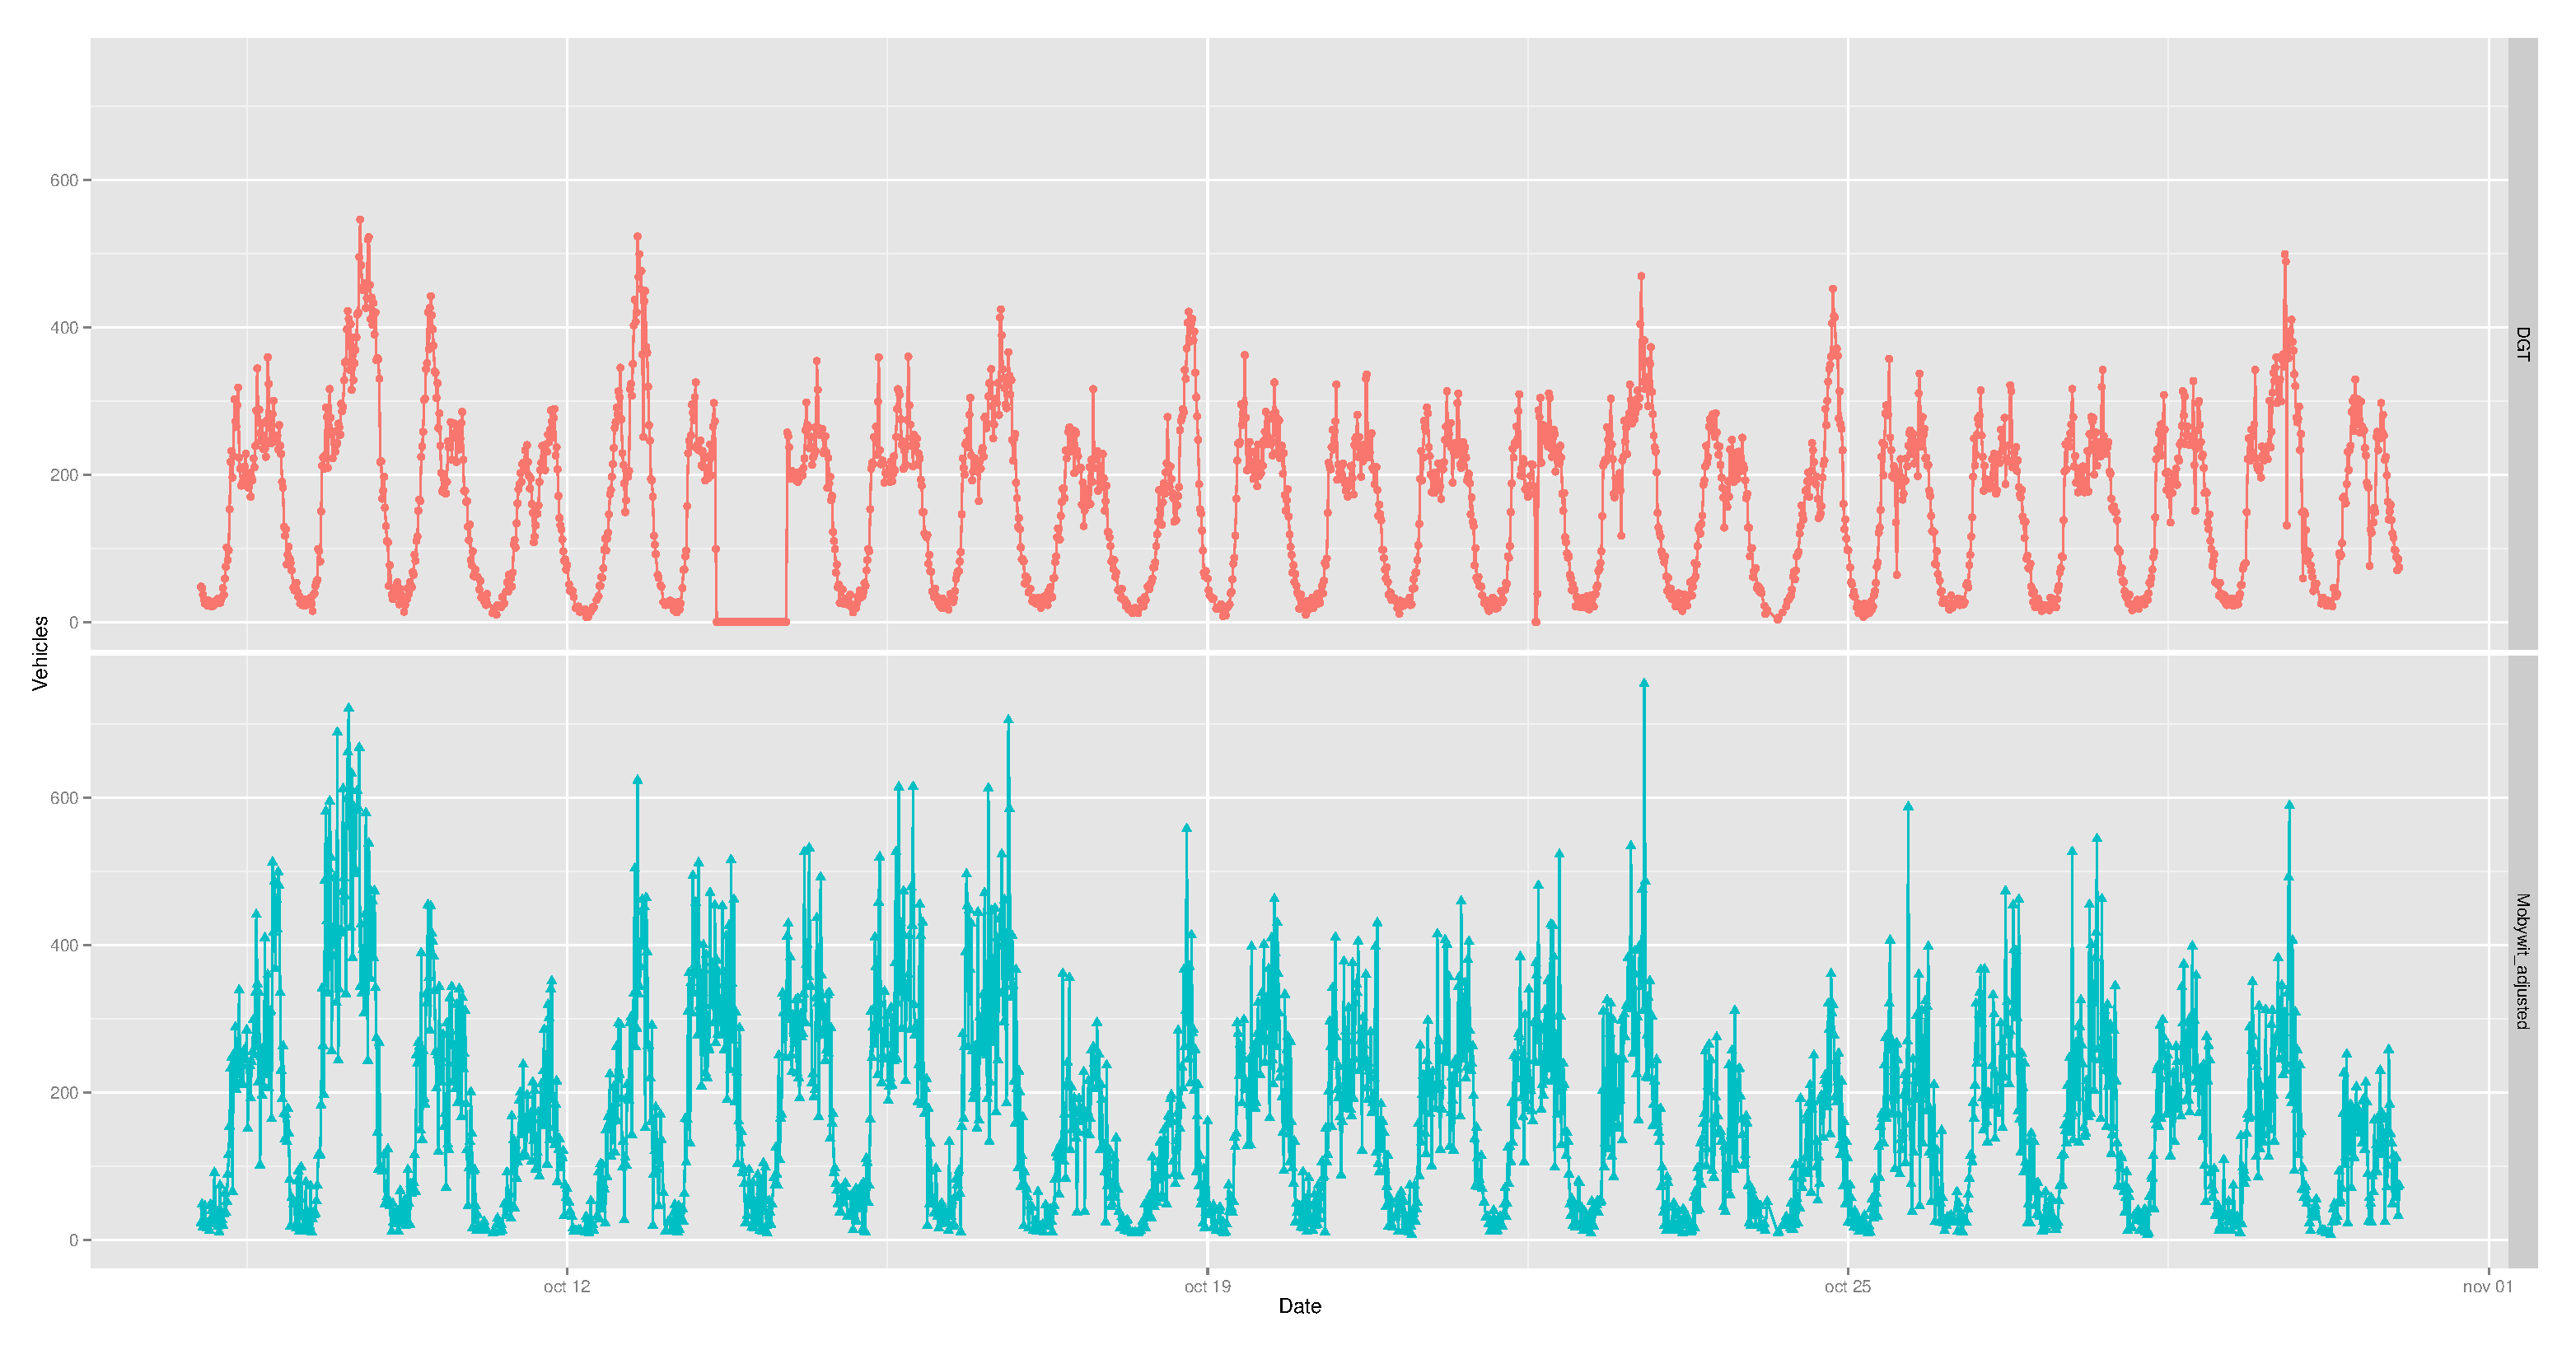
\includegraphics[scale=0.22]{imgs/petra_graph_DGT-Mobywit-mended.eps}
		\caption{Devices detected by DGT and detected by our device (node 1010) applying the correction ratio (median by quarter). Note: no DGT data available during October 14th.}
	\label{fig:dgtRatios}
	\end{center}
\end{figure}

\subsection{Context-sensitive nowcasting}
\label{ss:nc}

%----------------------------------------------------------------------------
%%%%%%%%%%%%%%%%%%%%%%%%%%%%%%%   CONCLUSIONS  %%%%%%%%%%%%%%%%%%%%%%%%%%%%%%%
%----------------------------------------------------------------------------

\section{Conclusions}
\label{sec:conclusions}

`holes' in the detected `events' when there is a power cutoff on a device.

%%%%%%%%%%%%%%%%%%%%%%%%%%%%%  ACKNOWLEDGEMENTS %%%%%%%%%%%%%%%%%%%%%%%%%%%%%%%%

\section*{Acknowledgements}

This work has been supported in part by projects EPHEMECH
(TIN2014-56494-C4-3-P, Spanish Ministry of Economy and Competitivity),
PETRA (SPIP2014-01437, funded by Direcci�n General de Tr�fico),
PYR-2014-17 (GENIL project, awarded by CEI-BIOTIC Granada), and MOSOS
(This work has been supported by the project with reference PRY142/14,
which has been granted by Fundaci�n P�blica Andaluza Centro de
Estudios Andaluces in the call 'IX Convocatoria de Proyectos de
Investigaci�n). We also thank the DGT and their staff and researchers for their dedication and
professionalism.  


% ---------------------- BIBLIOGRAF�A -----------------------

\bibliographystyle{elsarticle-num}
\bibliography{mobility,geneura-latin1}


\end{document}
